\documentclass[a4paper,10pt]{article}

%Math
\usepackage{amsmath}
\usepackage{amsfonts}
\usepackage{amssymb}
\usepackage{amsthm}
\usepackage{ulem}
\usepackage{stmaryrd} %f\"{u}r Blitz!

%PageStyle
%\usepackage[utf8x]{inputenc}
\usepackage[german]{babel}
\usepackage{fontenc}
\usepackage{fancyhdr, graphicx}
\usepackage[dvips]{hyperref}
\usepackage{wasysym}
\usepackage{fullpage}
\usepackage{textcomp}
\usepackage{fancyhdr} %for header/footer

%Zeichnung
\usepackage{tikz}
\usepackage[all]{xy}

\usepackage{color}
\usepackage{xcolor}
\usepackage{listings}

\usepackage{caption}
\DeclareCaptionFont{white}{\color{white}}
\DeclareCaptionFormat{listing}{\colorbox{gray}{\parbox{\textwidth}{#1#2#3}}}
\captionsetup[lstlisting]{format=listing,labelfont=white,textfont=white}

%lstlisting for java
\usepackage{listings}
  \usepackage{courier}
 \lstset{
         basicstyle=\footnotesize\ttfamily, % Standardschrift
         %numbers=left,               % Ort der Zeilennummern
         numberstyle=\tiny,          % Stil der Zeilennummern
         %stepnumber=2,               % Abstand zwischen den Zeilennummern
         numbersep=5pt,              % Abstand der Nummern zum Text
         tabsize=2,                  % Groesse von Tabs
         extendedchars=true,         %
         breaklines=true,            % Zeilen werden Umgebrochen
         keywordstyle=\color{red},
    		frame=b,         
 %        keywordstyle=[1]\textbf,    % Stil der Keywords
 %        keywordstyle=[2]\textbf,    %
 %        keywordstyle=[3]\textbf,    %
 %        keywordstyle=[4]\textbf,   \sqrt{\sqrt{}} %
         stringstyle=\color{white}\ttfamily, % Farbe der String
         showspaces=false,           % Leerzeichen anzeigen ?
         showtabs=false,             % Tabs anzeigen ?
         xleftmargin=17pt,
         framexleftmargin=17pt,
         framexrightmargin=5pt,
         framexbottommargin=4pt,
         %backgroundcolor=\color{lightgray},
         showstringspaces=false      % Leerzeichen in Strings anzeigen ?        
 }
 \lstloadlanguages{% Check Dokumentation for further languages ...
         %[Visual]Basic
         %Pascal
         %C
         %C++
         %XML
         %HTML
         Java
 }

%My Commands
\newcommand{\RN}{\mathbb{R}} %Real Number
\newcommand{\NN}{\mathbb{N}} %Natural Number
\newcommand{\QN}{\mathbb{Q}} %Rational Number
\newcommand{\ZN}{\mathbb{Z}} %ganze Zahlen
\newcommand{\CN}{\mathbb{C}}
\newcommand{\PN}{\mathbb{P}}
\newcommand{\EN}{\mathbb{E}}
\newcommand{\Teilt}{\mid} %|
\newcommand{\Teiltn}{\nmid} %kein teiler
\newcommand{\Potp}{\mathcal{P}} %Potenzmenge
\newcommand{\Pota}{\mathcal{A}}
\newcommand{\Potr}{\mathcal{R}}
\newcommand{\Potn}{\mathcal{N}}
\newcommand{\Bold}[1]{\textbf{#1}} %Boldface
\newcommand{\Kursiv}[1]{\textit{#1}} %Italic
\newcommand{\T}[1]{\text{#1}} %Textmode
\newcommand{\Nicht}[1]{\T{\sout{$ #1 $}}} %Streicht Shit durch
\newcommand{\lra}{\leftrightarrow} %Arrows
\newcommand{\ra}{\rightarrow}
\newcommand{\la}{\leftarrow}
\newcommand{\lral}{\longleftrightarrow}
\newcommand{\ral}{\longrightarrow}
\newcommand{\lal}{\longleftarrow}
\newcommand{\Lra}{\Leftrightarrow}
\newcommand{\Ra}{\Rightarrow}
\newcommand{\La}{\Leftarrow}
\newcommand{\Lral}{\Longleftrightarrow}
\newcommand{\Ral}{\Longrightarrow}
\newcommand{\Lal}{\Longleftarrow}
\newcommand{\Vektor}[1]{\vec{#1}}
\newcommand{\Brace}[1]{\left( #1 \right)} %()
\newcommand{\Bracel}[1]{\left\lbrace #1 \right.} %(
\newcommand{\Bracer}[1]{\right. #1 \right\rbrace} %)
\newcommand{\Brack}[1]{\left\lbrace #1 \right\rbrace} %{}
\newcommand{\Brackl}[1]{\left\lbrace #1 \right.} %{
\newcommand{\Brackr}[1]{\right. #1 \right\rbrace} %}
\newcommand{\Result}[1]{\underline{\underline{#1}}} %Doppelt unterstrichen
\newcommand{\Abs}[1]{\left| #1 \right|} %Absolutbetrag
\newcommand{\Norm}[1]{\Abs{\Abs{ #1 }}} %Norm
\newcommand{\Arrays}[1]{\left(\begin{array}{c}#1\end{array}\right)} %Array mit einer Kolonne ()
\newcommand{\Array}[2]{\left(\begin{array}{#1}#2\end{array}\right)} %Array mit n Kolonnen ()
\newcommand{\Bracka}[2]{\left\lbrace\begin{array}{#1}#2\end{array}\right\rbrace} %Array mit {}
\newcommand{\Brackal}[2]{\left\lbrace\begin{array}{#1} #2 \end{array}\right.} %Array mit {
\newcommand{\Brackar}[2]{\left.\begin{array}{#1} #2 \end{array}\right\rbrace} %Array mit }
\newcommand{\Sumone}[2]{\sum_{#2=1}^{#1}} %Summe von 1
\newcommand{\Sumz}[2]{\sum_{#2=0}^{#1}} %Summe von 0
\newcommand{\Sum}[2]{\sum_{#2}^{#1}} %Allgemeine Summe
\newcommand{\Oneover}[1]{\frac{1}{#1}} %1 \"{u}ber igendwas
\newcommand{\Tablewt}[3]{\begin{table*}[h]\caption{#1} \begin{tabular}{#2}{#3}\end{tabular}\end{table*}} %Table mit Titel
\newcommand{\Oben}[2]{\overset{#1}{#2}} %etwas \"{u}ber etwas anderem
\newcommand{\Unten}[2]{\underset{#1}{#2}} %etwas unter etwas anderem
\newcommand{\Bildcap}[2]{\begin{figure}[htb]\centering\includegraphics[width=0.2\textwidth]{#1} \caption{#2}\end{figure}} %Bild mit beschriftung
\newcommand{\Bildjpeg}[1]{\includegraphics[width=0.2\textwidth]{#1.jpeg}} %Bilder jpeg!!
\newcommand{\Bildjpg}[1]{\includegraphics[width=0.2\textwidth]{#1.jpg}} %Bilder jpg!!
%Beispiel f\"{u}r lstlisting \lstinputlisting[label=Aufgabe 4a,caption=Aufgabe 4a]{4a.java}

\usepackage{ucs}
\author{Fabio Oesch}
\title{Wahrscheinlichkeiten und Statistik}

\begin{document}
\maketitle
\pagebreak
\tableofcontents
\pagebreak
\section{Themen}
\begin{enumerate}
 \item beliebig oft wiederholbar
 \item Resultat ist zuf\"{a}llig
\end{enumerate}
\Bold{Bsp:} Lotto, M\"{u}nze werfen, W\"{u}rfeln
\subsection{Ergebnisraum}
$\Omega$ = Menge aller m\"{o}glichen Ausg\"{a}nge des Experiemnts (im Skript mit $S$)\\
\Bold{Bsp:} $\Omega$ von Lotto: $\Omega=\{1,\dots,45\}$\\
\subsection{Ereignis $E\subseteq\Omega$}
Ereignis $E=$\{Augenzahl ist gerade\}\\
spezielle Ereignisse:
\begin{itemize}
 \item $E=\Omega$ sicheres Ereignis
 \item $E=\emptyset$ unm\"{o}gliches Ereignis
\end{itemize}
$E$ Ereignis: $E^C=\overline{E}=\Omega\backslash E$
\subsection{Wahrscheinlichkeitsfunktion}
$\PN:\Potp(\Omega) \to[0,1]$\\
2 wichtige Eigenschaften: $\Potp(\Omega) = 1$, $\Potp(\emptyset)=0$, $0\leq\Potp(E)\leq1$\\
\Bold{Bsp:} $\Omega = \{$Kopf, Zahl, Kante$\}$\\
$\Brackar{l}{\Potp(\{\T{Kopf}\}=\frac{2}{3}\\
\Potp(\{\T{Kante}\}=0\\
\Potp(\{\T{Zahl}\}=\Oneover{3}}\Ra\Potp(E)=1$, $E=\{\T{Kopf, Zahl}\}$
\subsection{Subaditivit\"{a}t}
$E_1$, $E_2\subseteq \Omega$, $E_1\cap E_2=\emptyset\Ra \Potp(E_1\cup E_2)=\Potp(E_1)+P(E_2)$\\
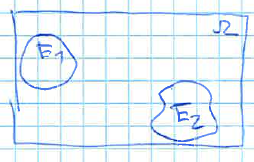
\includegraphics[scale=0.5]{Pic2.png}$\Ra\Potp(E_1\cup E_2)=\Potp(E_1)+\Potp(E_2)$, $E=E_1\cup E_2$\\
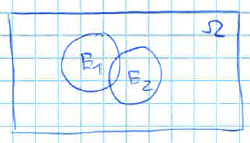
\includegraphics[scale=0.5]{Pic3.png}$\Ra\Potp(E)=\Potp(E_1)+\Potp(E_2)-\Potp(E_1\cap E_2)$, $E=E_1\cup E_2$\\
$\Potp(E_1\cup E_2 \cup \dots \cup E_n)\leq \Potp(E_1)+\dots+\Potp(E_n)$\\
\Bold{Bsp:} Lotto mit Matryoshka\\
$\Potp(\{w\})=\Oneover{45}$, $E_1 =\{1\}$, $E_2=\{1,2\}$, $\dots$, $E_{45}=\{1,\dots,45\}=\Omega\Ra \Potp\overbrace{(E_1\cup\dots\cup E_{45})}^{\Omega}=1$\\
$\Potp(E_1\cup E_2\cup \dots\cup E_{45}\leq\Potp(E_1)+\dots+\Potp(E_{45})=\Oneover{45}+\frac{2}{45}+\dots+\frac{45}{45}=\frac{\frac{45\cdot46}{2}}{45}=\frac{46}{2}=23$\\
\subsection{Wahrscheinlichkeitsraum (Vorl\"{a}ufig)}
$W=(\Omega$, $\Potp(\Omega)$, $\PN)$, $\Omega=$ Ergebnisraum, $\Potp(\Omega)=$alle Ausg\"{a}nge des Experiments. alle $E$'s, $\PN=$ Wahrscheinlichkeitsfunktion
\subsection{Theoretische Wahrscheinlichkeitsfunktion}
$\Potp($\{Zahl\}$)=\Potp($\{Kopf\}$=\Oneover{2}$ (Definiere die Wahrscheinlichkeit synthetisch)\\
$\Pota(E)=\frac{\T{wie h\"{a}ufig tritt }E\T{ ein bei N-facher Wiederholung}}{N}$ (Empirische Wahrscheinlichkeit)
\subsection{Laplace-Experimente}
$\underline{\wedge}$ Fairen Spielen, Die Wahrscheinlichkeiten sind gleichverteilt\\
$\Abs{\Omega}=n$ endlicher Wahrscheinlichkeitraum.\\
Jedes Elementarergebnis ist gleich wahrscheinlich $(\Abs{E}=1)$. \Bold{Bsp:} W\"{u}rfel: $\{1\}=\{1,2,3,4,5,6\}$. kein Elementarergebnis: $\{3,4\}$
$\omega\in\Omega:\Potp(\{\omega\})=\Oneover{n}=\Oneover{\Abs{\Omega}}$, $\Abs{A}$= Anzahl Elemente in $A$
\subsection{Mehrstufige Zufallsexperiment}
Zufallsexperiment $Z$, das mehrfache hintereinander angef\"{u}hrt wird.\\
\Bold{Bsp:} mehrmals W\"{u}rfeln: Wie gross ist die W'keit $2\times$ hintereinander 6 zu w\"{u}rfeln: $\Potp(2\times $ 6 W\"{u}rfeln$)=\Oneover{36}$\\
Produktregel: $\Potp(E_1$ und $E_2)=\Potp(E_1)\cdot \Potp(E_2)$\\
M\"{o}glichkeiten: $\Omega_1$ hat $n_1$ viele Ausg\"{a}nge $(\Abs{\Omega_1}=n_1)$, $\Omega_2$ hat $n_2$ viele Ausg\"{a}nge $(\Abs{\Omega_2}=n_2)$ also $n_1\cdot n_2$
\subsection{Urnenmodel}
Unterscheidung nach "`Zur\"{u}cklegen"' oder "`nicht zur\"{u}cklegen"' und "`geordnet"' oder "`keine Reihenfolge"'
\begin{tabular}{l|l|l}
 &zur\"{u}cklegen&nicht zur\"{u}cklegen\\\hline
 geordnet&$n^k$&$n!$ oder $\frac{n!}{(n-k)!}$\\\hline
 ungeordnet&&$\binom{n}{k}=\frac{n!}{k!(n-k)!}$
\end{tabular}\\
$p=\frac{\T{Anzahl der günstigen Fälle}}{\T{Anzahl der möglichen Fälle}}=\frac{g}{m}$\\
\Bold{Bsp:} Klasse aus 10 M\"{a}dchen und 14 Knaben. W\"{a}hle 5 Personen aus.\\
a) W'keit, dass alle M\"{a}dchen sind?\\
Antwort: $P(\{5\T{ M\"{a}dchen}\})=\frac{\Abs{\{5\T{ M\"{a}dchen}\}}}{\Abs{\Omega}}$, $\Abs{\Omega}={24 \choose 5}$, $\Abs{\{5\T{ M\"{a}dchen}\}}={10\choose5}$\\
$\Ra P(\{5\T{ M\"{a}dchen}\})=\frac{{10\choose5}}{{24\choose5}}$\\\
b) W'keit alles Knaben: $P(\{5\T{ Knaben}\})=\frac{{14\choose5}}{{24\choose5}}$\\
c) W'keit, dass in der 5-er Gruppe, sowohl M\"{a}dchen, als auch Knaben vorkommen.\\
Gegenw'keit von a) + b), also $\overline{E}=\{$nur M\"{a}dchen oder nur Knaben$\}\Ra P(\overline{E})=P(\{$nur M\"{a}dchen$\})+P(\{$nur Knaben$\})=\frac{{10\choose5}+{14\choose5}}{{24\choose5}}\Ra P(E)=1-P(\overline{E})$\\
\Bold{Gegenw'keit benutzen:} $P(E)$, $\frac{\Omega}{E}=\overline{E}$, $1-P(\overline{E})=P(E)$\\
\Bold{Bsp:} 8x M\"{u}nze werfen\\
Wie gross ist die W'keit, das Zahl \& Kopf gleichh\"{a}ufig vorkommen.\\
$\Abs{E}={8\choose4}\cdot{4\choose4}$
\subsection{Repetition}
$\Brackar{l}{
X\T{ Zufallsvariable: Anzahl bei 1x w\"{u}rfeln}\\
Y\T{ Zufallsvariable: Anzahl bei 1x w\"{u}rfeln}}$
$X,Y$ Gleichverteilt (uniform) uniform\\
$Z:=X+Y$ Zufallsvariable: $F(z)=\Sum{}{X_i\leq Z}p_i$, $p_i =P(Z=x_i)$\\
\subsection{Erwartungswert:}
Theoretischer Pendant zum Mittelwert.\\
\Bold{Bsp:} $x_1,x_2,x_3,x_4$, $h=\Abs{\{x_1,x_2,x_3,x_4\}}$ $\ra$ $\overline{x}=\frac{\Sum{}{}x_i}{h}$\\
$\EN X=\mu=\Sum{}{\T{alle }X_i}x_i\cdot\PN(X=x_i)$ keine Zufallsvariable\\
\Bold{Bsp:} $X$ sein die Augenzahl von 1x w\"{u}rfeln. $\EN X=\Sum{6}{i=1}i\cdot \frac{1}{6}=3.5$\\
$Y=X-\EN(X)$ ist eine Zufallsvariable, $\EN Y=\EN(X-\EN X)=\Sum{n}{i=1}(x_i p_i-p_i\EN(X))=\Sum{n}{i=1}x_ip_i-\Sum{n}{i=1}p_i\EN(X)=\EN(X)-\EN(X)\Sum{n}{i=1}p_i=\EN(X)-\EN(X)=0$\\
\Bold{Bsp: W\"{u}rfel} $\EN(X)=3.5$, $E(X-\EN(X))=0$\\
\begin{tabular}{c|c|c|c|c|c|c}
 $X-3.5$&$1-3.5$&$2-3.5$&$3-3.5$&$4-3.5$&$5-3.5$&$6-3.5$\\\hline
 $p_i$&$\frac{1}{6}$&$\frac{1}{6}$&$\frac{1}{6}$&$\frac{1}{6}$&$\frac{1}{6}$&$\frac{1}{6}$
\end{tabular}
\subsection{Streuung, Varianz}
Var$(X):=\EN((X-\EN(X))^2) \Ra \EN(X-\mu)^2=\EN(X^2)-\EN(X)^2$
\subsection{Binomialverteilung}
Zufallsexperiment mit 2 Ausg\"{a}ngen: Erfolg, Misserfolg\\
$P(X=\T{Erfolg})=p\in[0,1]$, $P(X=\T{Misserfolg})=1-p=q$\\
Zufallsvariable $X=$ Anzahl Erfolge bei $n$-facher Wiederholung des Experiments\\
Wahrscheinlichkeitsfunktion von $X$ aus. $P(X=x)=$
\begin{tabular}{c|ccccc}
 $x_i$&0&1&$k$&$n$\\\hline
 $p_i$&$(1-p)^n$&${n\choose1}p(1-p)^{n-1}$&${n\choose k}p^k(1-p)^{n-k}$&${n\choose n}p^n$
\end{tabular}\\
\Bold{Bsp:}\\
Spieler A: M.D. 40\% Erfolgsw'keit, Spieler B: K.G. 60\% Erfolgsw'keit.\\
Sie spielen 3x gegeneinander. E: W'keit dass A h\"{a}ufiger als B gewinnt. Also muss A 2- oder 3-Mal gewinnen.
$P(X=2)+P(X=3)\Ra {3\choose2}0.4^2\cdot0.6+{3\choose3}0.4^3+0.6^0=0.352\Ra35.2$\% W'keit gewinnt $A$\\
Erfolgsw'keit von $p$: $\EN X$ bei $n$ spielen. Mit Trick: $\EN X=n\cdot p$\\
$(a+b)^n=\Sumz{n}{k}{n\choose k}a^kb^{n-k}$\\
$f(t)=(q+pt)^n=\Sumz{n}{k}{n\choose k}q^{n-k}(pt)^k$\\
\subsubsection{Binomialverteilung:}
Abk\"{u}rzung: $X\sim$ Bin$(n,p)$, $n$: Anzahl Experimente, $p$: Erfolgsw'keit\\
$P=(X=k)={n\choose k}p^k(1-p)^{n-k}$, $\EN(X)=np$, Var$(X)=\sigma^2=np(1-p)$. $\sigma$: Std'abweichung
\subsubsection{Testen einer Hypothese:}
Vermutung: H\"{u}hner k\"{o}nnen zw. $\circ$ und $\vartriangle$ Futter entscheiden.\\
$20\times\circ$, $20\times\vartriangle$ $\Ra$ $\circ=$ Erfolg, $\vartriangle=$ Misserfolg\\
Zufallsvariable $X$ z\"{a}hlt die Anzahl Erfolge $\Ra$ Binomiales Experiment d.h. $X\sim\T{Bin}(20,p)$.\\
F\"{u}hren das Experiment durch: $15\times\circ$ und $5\times\vartriangle$, experimentelle W'keit f\"{u}r Erfolg: $p=\frac{15}{20}=\frac{3}{4}$\\
\Bold{Hypothese formulieren:}\\
$H_0$: Nullhypothese: es gibt keinen Unterschied $\ra$ Huhn kann nicht unterscheiden zw. $\circ$ \& $\vartriangle$, $p=q=\Oneover{2}$\\
$H_1$: Alternativhypothese: $p\geq q$ ($p\leq q$). d.h. es gibt einen Unterschied beim Fressverhalten.\\
\Bold{Ziel:} Entscheiden ob $H_0$ anzunehmen ist, oder sie zugunsten von $H_1$ verwerfen.\\
\Bold{Berechnung:} Berechne W'keit unter $H_0(p=q=\Oneover{2})$, dass wir einen Ausgang mit $15\times$ Erfolg und $5\times$ Misserfolg\\
$P(15\leq X\leq20)=\Sum{20}{k=15}{20\choose k}p^k(1-p)^{20-k}\Oben{\T{unter }H_0!}{=}\Sum{20}{k=15}{20\choose k}\Oneover{2}^k\cdot\Oneover{2}^{20-k}\approx0.021=2.1\%$, Signifikanz-Niveau $\alpha$, $\alpha=0.1$ ($10\%$) $\Ra$ Falls $P(15\leq X\leq 20|H_0)\leq\alpha\Ra$ dann verwerfen $H_0$, ansonsten nehmen wir $H_0$ an.\\
$\bullet$ 2 M\"{o}glichkeiten: falls unter der Nullhypothese 
\begin{enumerate}
 \item $P(15\leq X\leq 20)>\alpha$, dann nehmen wir die Nullhypothese an es spricht nichts gegen $H_0$ auf Signifikanzniveau $\alpha$
 \item $P(15\leq X\leq 20)\leq \alpha$, dann verwerfen wir $H_0$ zugunsten von $H_1$
\end{enumerate}
$\bullet$ (2) Fehler 1. Art; verwerfen von $H_0$, obwohl $H_0$, obwohl $H_0$ korrekt w\"{a}re $\ra$ Irrtumsw'keit $P(15\leq X\leq 20)$.\\
$\bullet$ (1) Fehler 2. Art; verwerfen $H_1$, obwohl $H_1$ korrekt ist $\ra$ Irrtumsw'keit $\beta$ (Power)
\subsection{Poissonverteilung}
\begin{enumerate}
 \item Gleichverteilung (fairer Würfel)
 \item Binomialverteilung
 \item Poissonverteilung
\end{enumerate}
\Bold{Idee:} $p$ soll sehr klein sein. $n$ soll sehr gross sein.\\
\Bold{Bsp:} $X$ sei binomialverteilt und Parametern $n$, $p$. $\Ra\EN(X)=n\cdot p$.\\
$\lim_{n\to\inf}n\cdot p_n=\lambda\in\RN$, $\Ra p=\frac{\lambda}{n}$\\
$X$ binomialverteilt: $P(X=k)={n\choose k}\cdot p^k(1-p)^{n-k}$, $\Oben{?}{\Ra}$ $\lim_{n\to\inf}P(X=k)=\frac{\lambda^k}{k!}\cdot e^{-\lambda}$\\
Verteilung mit W'keitsfunktion $\frac{\lambda^k}{k!}\cdot e^{-\lambda}$ heisst Poissonverteilung.\\
Erwartungswert von $X\tilde Poi(\lambda)$ ($X$ ist Poisson-verteilung mit Parameter $\lambda$)\\
$\EN(X)=\Sumz{\infty}{x}x\cdot P(X=x)=\lambda$
\begin{itemize}
 \item Für sehr kleine W'keiten. Mit bekanntem "`Mittelwert"' (Erwartungswert) $\lambda$. Mit quasi unendlich (unbekannter) Anzahl gleicher Experimente.
 \item $P(X=x)=\frac{\lambda^xe^{-lambda}}{x!}$
 \item $\EN(X)=\lambda$
 \item Var$(X)=\lambda$
 \item $X\tilde Poi(\lambda)$, $Y\tilde Poi(\mu)$, $Z=X+Y:$ $Z\tilde Poi(\lambda+\mu)$
\end{itemize}
\Bold{Bsp:} Smartphonehersteller, Fehlerquote von $1\textperthousand$, $5.000$ Smartphones\\
Wie gross ist die W'keit, dass mind. 2 defekt sind.\\
Poissonapproximation: $\lambda = 0.001\cdot 5000=5$\\
$P(X\geq 2)=1-(P(X=1)+P(X=0))=1-(\frac{\lambda^1e^{-\lambda}}{1!}+\frac{\lambda^0e^{-\lambda}}{0!})=1-(\frac{5^1e^{-5}}{1!}+\frac{5^0e^{-5}}{0!})=1-6e^{-5}\approx 0.96$
\subsection{Statistische Tests}
\subsubsection{Prinzip des statistischen Tests}
\begin{enumerate}
 \item Nullhypothese $H_0$ formulieren. \\
Bsp: $\Brackar{r}{H_0:p=\Oneover{6}\T{ bei einem Würfel}\\
 H_1:p>\Oneover{6} \T{ Alternativhypoth.}}H_1\cap H_0=\emptyset$
 \item Signifikanzniveau $\alpha\in(0,1)$
 \item Stichprobe sammeln
 \item Entscheid fällen: Berechne W'keit unter $H_0$, das wir einen Ausgang haben, wie die Stichprobe\\
 Ist sie grösser als $\alpha\Ra H_0$ annehmen\\
 Ist sie kleiner als $\alpha\Ra H_0$ zugunsten von $H_1$ verwerfen
\end{enumerate}
\subsubsection{Beispiel}
12'000 mal Würfeln, 2'107 mal Sechs, $\alpha=10\%$
\begin{itemize}
 \item $H_0: p=\Oneover{6}$ Nullhypothese
 \item $H_1:p>\Oneover{6}$ Alternativhypothese
\end{itemize}
$\EN(X)=np=12000\cdot\Oneover{6}=2000$\\
Wir berechnen die Wahrscheinlichkeit von $P(2107\leq X)$. Wir benötigen Grenzwertsatz von de Moivre und Laplace. $\mu=np=12000\cdot\Oneover{6}=2000$ und $\sigma^2=np(1-p)=12000\cdot\Oneover{6}\cdot\frac{5}{6}=1666\frac{2}{3}$. Die Approximation ist erlaubt, da die Faustregel $np(1-p)=1666\frac{2}{3}>9$ erfüllt ist.\\
Nun erhalten wir mit der Tafel:\\
$P(2107\leq X)\approx1-\Phi(\frac{2107-2000}{\sqrt{1666\frac{2}{3}}},0,1)=1-\Phi(2.621,0,1)=1-0.9956=0.0044$\\
Da $\alpha<0.0044$ ist verwerfen wir $H_0$
\subsubsection{Erwartungswert und Varianz}
Auf dem Intervall $I=]-\infty,\infty[$\\
Erwartungswert $\mu=\EN(X)=\int_{x_1}^{x_2}xf(x)dx$, Varianz $\sigma^2=\int_{x_1}^{x_2}x^2f(x)dx-\mu^2$
\subsection{t-Verteilung}
$X_1,\dots,X_n\sim N(\mu,\sigma^2)$\\
$T_{n-1}:=\frac{\Oneover{n}\Sumone{n}{i}X_i-\mu}{\sqrt{\Oneover{n-1}\Sumone{n}{i}(X_i-\mu)^2}}\sqrt{n} \in\RN^{\Omega^n}$ heisst t-verteilt mit $n-1$ Freiheitsgraden\\
$t_{n-1}:=\frac{\Oneover{n}\Sumone{n}{i}x_i-\mu}{\sqrt{\Oneover{n-1}\Sumone{n}{i}(x_i-\bar{x})^2}}\sqrt{n}\in\RN$\\
$f_{n-1}(t)=c_{n-1}(1+\frac{t^2}{n})^-{\frac{n+1}{2}}$ für $\lim_{n\to\infty}\to\varphi(t,0,1)$\\
$c_{n-1}=\frac{\Gamma(\frac{n}{2})}{\sqrt{\pi(n-1)}\Gamma(\frac{n-1}{2})}$, $\Gamma(x)=\int_0^\infty t^{x-1}e^{-t}dt$. Gammafunktion.\\
$\Gamma(x+1)=x\Gamma(x)$; $\Gamma(1)=1$; $\Gamma(5)=\Gamma(4+1)=4\Gamma(4)=4\Gamma(3+1)=4\cdot3\cdot\Gamma(3)=\dots=5!$\\
\subsection{Parametertests}
\begin{itemize}
 \item 1-Stichprobentest\\
$H_0:\mu=\bar{x}$ $X\sim W(\mu_1,\sigma_1^2)$
$H_1:\mu\neq\bar{x}$ $Y\sim W(\mu_2, \sigma_2^2)$
 \item 2-Stichprobentest\\
$H_0:\mu_1\neq\mu_2$
\end{itemize}
Grundvoraussage:
\begin{itemize}
 \item Verteilungsfamilie bekannt\\
 (d.h. $W(\cdot,\cdot)$, t-verteilt, Weibull etz)
 \item Testen ob 
1-Stichpr.fall $H_0:\vartheta=\hat{\vartheta}_n$ ($\vartheta$: fester Wert, $\hat{vartheta}$: empirisch)\\
2-sTichpr.fall $H_0:\hat{\vartheta}_n=\hat{\vartheta}_m$
\end{itemize}
\begin{enumerate}
 \item Verteilung von $T_n$ (Teststatistik) unter $H_0$ bekannt $\Lra:$ exakter Test.
 \item Verteilung von $T_n$ unter $H_0$ unbekannt.
\end{enumerate}
Nicht parametrische Tests (Verteilungsfreie Tests):
\begin{itemize}
 \item 1./2. Stichprobentests existieren
 \item keine Verteilungsparameter
\end{itemize}
1. Stichprobentest $H_0:\hat{F_n}(x)=F_0(x)$\\
2. Stichprobentest $H_0:\hat{F_n}(x)=\hat{G_m}(x)$\\
$\bar{F_n}(x)=\Oneover{n}\Sumone{n}{i}\mathbb{I}\{x_i\leq x\}$
\subsection{Konfidenz/Vertrauensintervall}
$X\sim N(\mu,\sigma^2)$\\
Experiment $n$-mail durchführen. $\Ra X=\{x_1,\dots,x_n\}$\\
Theoretisch $\EN(X)=\mu$\\
Empirisch: $\bar{x}=\Oneover{n}\Sumone{n}{i}x_i$ als Schätzung von $\mu$\\
Wie gut ist die Schätzung? Vorgabe: $\gamma\in[0,1]$\\ $[\mu-\vartriangle x,\mu+\vartriangle x]\ni \bar{x}$ Finde $\vartriangle x$, so dass $\mathbb{P}(\bar{x}\in[\mu-\vartriangle x,\mu+\vartriangle x]=\gamma$.\\
$\bar{x}=\Oneover{n}\Sumone{n}{i}x_i$. $s^2=\Oneover{n-1}\Sumone{n}{i}(x_i-x)^2$. $t_{n-1}=\frac{\bar{x}-\mu}{s}$ (t-verteilt (exakt) für ZV.).\\
$\mathbb{P}(\bar{x}\in[\mu-\vartriangle x,\mu+\vartriangle x])=\gamma=1-\alpha$\\
\Bold{Beispiel:}
$n=10$ Stichproben $X=\{x_1,\dots,x_n\}$\\
$\bar{x}=5$. $s=0.2$ Vertrauensintervall $=?$ bei Vertraunsw'keit von $\gamma=0.95\Ra \alpha=0.05$; $1-\frac{\alpha}{2}=1-0.025=0.975$\\
$\Ra\vartriangle x=\frac{t_{10-1},0.975}{\sqrt{10}}\cdot 0.2$ Tabelle betrachten Seite 140 ergibt mit Freiheitsgrad $=n-1=9$. $t_{9,0.975}=2.262$.\\
$\Ra \vartriangle x=\frac{2.262}{\sqrt{10}}\cdot 0.2\approx 0.14$\\
Vertrauensintervall $[4.86, 5.14]$. mit W'keit von $95\%$ liegt $\mu$ in $[4.86, 5.14] = [5-\vartriangle x, 5+\vartriangle x]$\\
\Bold{Allgemein}\\
Feste Vertrauensw'keit $\gamma=0.95$\\
$s$ konstant\\
Stichproben $n$: $\vartriangle x=\frac{t_{N-1,0.975}}{\sqrt{N}}s (n\to\infty)=0$\\
$t_{n,0.975}\leq t_{n-1,0.975}\leq2.262$ für $n\geq10$\\
\Bold{Beispiel:}\\
$t=\overbrace{\frac{\bar{x}-\mu}{s}}^{\vartriangle\mu}\sqrt{s}$\\
Festes $\gamma$, und $\vartriangle\mu$. Wie gross $n$ wählen?\\
$\frac{t\cdot s}{\bar{x}-\mu}=\sqrt{n}\Oben{^2}{\Ra}\frac{t^2\cdot s^2}{(\vartriangle x)^2}\leq n$\\
$\bullet$ Vorgehen: - Vertrauensintervallgrösse $\vartriangle\mu$, - Vertrauensw'keit $\gamma$ ($\to$ fliesst in $t$ ein)\\
$t=t_{n-1,1-\frac{1-\gamma}{2}}$ Quantifunktion der t-Verteilung.\\
$\bullet$ Abschätzung: $t\approx 2$ (oder $t=3)$. Daumenregel: $\frac{4\cdot s^2}{(\vartriangle\mu)^2}\geq N$ ($s^2$ ist geschätzt)
\subsubsection{2-Stichproben t-Test}
Annahme: $\bullet$ Normalverteilung, $\bullet$ 2 Gruppen\\
$H_0:\mu_1=\mu_2$, $H_1: \mu_1\neq\mu_2$\\
2 Fälle: a) unbekannte, aber gleiche Varianz d.h. $\sigma_1^2=\sigma_2^2=\sigma_2$ (Homoskedastisch) exakter Test\\
 b) unbekannte, evtl. ungleiche Varianzen, $\sigma_1^2\neq\sigma_2^2$ (Heteroskedastisch) approximation
\subsubsection{Homoskedastischer Fall}
Zwei Stichproben: $X=\{x_1,\dots,x_n\}$ $W(\mu,\sigma^2)$; $Y=\{y_1,\dots,y_n\}$ $W(\mu_2,\sigma^2)$\\
$\mu_1,\mu_2,\sigma^2$ sind unbekannt.\\
Testen, ob $\mu_1=\mu_2$ auf Signifikanzniveau $\alpha$ (2-seitiger Test, d.h. $H_0:\mu_1=\mu_2$ gegen $H_1:\mu_1\neq\mu_2$)\\
Testgrösse: $t=\frac{\bar{x}-\bar{y}}{s}\sqrt{\frac{n\cdot m}{n+m}}$. t-verteilt mit $n+m-2$ Freiheitsgraden\\ 
$\bar{s_1}=\Oneover{n-1}\Sumone{n}{i}(x_i-\bar{x})^2$, $\bar{m-1}=\Oneover{m}\Sumone{m}{i}(y_i-\bar{y})^2$\\
$s=\frac{(n-1)s_1^2+(m-1)s_2^2}{n+m-2}=\frac{\Sumone{n}{i}(x_i-\bar{x})^2+\Sumone{m}{i}(y_i-\bar{y})^2}{n+m-2}$\\
Signifikanzniveau $\alpha$: Ist $\Abs{t} < t_{n+m-2,1-\frac{\alpha}{2}}\Ra H_0$ annehmen. Ist $\Abs{t} \geq t_{n+m-2,1-\frac{\alpha}{2}}\Ra H_0$ ablehnen.
\section{Beispiele:}
\Bold{Aufgabe 3.5.8.} Auf wie viele Arten k\"{o}nnen die Buchstaben des Wortes Pfeffer permutiert werden? $\frac{7!}{3!\cdot 2!}=420$\\
\Bold{Aufgabe 3.5.10.} Eine Klasse hat 15 Fussballspieler, einer davon heisst Klaus. Auf wie viele Arten kann eine Mannschaft von 11 Spielern a. Mit Klaus, b. ohne Klaus zusammengestellt werden. a. ${14\choose 10}$, b. ${14\choose 11}$\\
\Bold{Aufgabe 3.5.14.} Wie viele M\"{o}glichkeiten gibt es, die 36 Jasskarten auf vier Spieler $A$, $B$, $C$, $D$ zu verteilen? ${36\choose9}\cdot{27\choose9}\cdot{18\choose9}\cdot{9\choose9}$\\
\Bold{Aufgabe 4.1.3} von 10 Nüssen sind 3 verdorben. Wahrscheinlichkeit, dass 2 gute Nüsse genommen werden, $m={10\choose 2},g={7\choose2}\Ra p=\frac{{7\choose2}}{{10\choose2}}\frac{7}{15}$\\
\Bold{Aufgabe 4.1.12} 10 Lose 2 Gewinnlose mit 5x herausziehen genau 1 Gewinnlos $\Ra m=8,n=2,k=5,s=1\Ra \frac{{8\choose4}{2\choose1}}{{10\choose5}}$\\
\Bold{Aufgabe 4.1.13} Es liegen $m+n$ Lose vor, unter denen $n$ Gewinnlose sind. Es werden $k$ Lose auf einmal gezogen. Bestimmen Sie die W'keit daf\"{u}r, dass sich unter den $k$ Losen genau $s$ Gewinnlose befinden.\\
Es gibt $m={m+n\choose k}$ m\"{o}gliche Ausf\"{a}lle und genau $g={m\choose k-s}{n\choose s}$ M\"{o}glichkeiten f\"{u}r $s$ Gewinnlose. Dabei z\"{a}hlt der Faktor ${m\choose k-s}$ die M\"{o}glickeiten, $k-s$ Nieten zu haben und der Faktor ${n\choose s}$ z\"{a}hlt die M\"{o}glichkeiten, $s$ Treffer zu haben. Damit folgt $p(s)=\frac{{m\choose k-s}{n\choose s}}{{m+n\choose k}}$.\\
\Bold{Bsp:} Würfel für sechs $p=\Oneover{6}, p>\Oneover{6}$ a) 2x 6 in 3 Würfen b) 3x 6 in 5 Würfen\\
$H_0:p=\Oneover{6}$ mit $\alpha=5\%$ also gilt: a) $P(2\leq X\leq 3)={3\choose2}(\Oneover{6})^2(\frac{5}{6})^1+{3\choose3}(\Oneover{6})^3(\frac{5}{6})^0=0.074>\alpha\Ra H_0$ angenommen; b) $P(3\leq X\leq 5)={5\choose3}(\Oneover{6})^3(\frac{5}{6})^2+{5\choose4}(\Oneover{6})^4(\frac{5}{6})^1+{5\choose5}(\Oneover{6})^5(\frac{5}{6})^0=0.035<\alpha\Ra H_0$ nicht angenommen;


\end{document}
